% =====================================================================================================
% IEEE Access draft -- VaultTrust (BITE497J, VIT Vellore)
% Compile with the official IEEE Access LaTeX template (ieeeaccess.cls + its logo/bullet files), e.g.
% on Overleaf: open the "IEEE Access LaTeX Template", upload this file and the figures/ folder, and set
% main.tex as the main document. Every number below comes from reports/eval/*.json.
% Lines marked  %% TODO  need the authors' input before submission.
% =====================================================================================================
\documentclass{ieeeaccess}
\usepackage{cite}
\usepackage{amsmath,amssymb,amsfonts}
\usepackage{graphicx}
\usepackage{textcomp}
\usepackage{booktabs}
\usepackage{multirow}
\usepackage{url}

\newcommand{\pct}{\,\%}

\begin{document}
\history{Date of publication xxxx 00, 0000, date of current version xxxx 00, 0000.}
\doi{10.1109/ACCESS.2026.DOI}

\title{Transaction-Bound Step-Up Authentication for High-Value Payments: Randomized Liveness,
Cancelable Face Templates, and Random-Walk One-Time Passwords}

%% TODO: confirm author order, IEEE membership (if any) and the corresponding author with the guide.
\author{\uppercase{Nilay Kant Shahi}\authorrefmark{1},
\uppercase{Magizharasan K}\authorrefmark{1},
\uppercase{Rwitankar Giri}\authorrefmark{1}, and
\uppercase{Mohanraj G}\authorrefmark{1}}

\address[1]{School of Computer Science Engineering and Information Systems, Vellore Institute of
Technology, Vellore, Tamil Nadu 632014, India}  %% TODO: check the official school name and add e-mails

\tfootnote{This work received no external funding.}  %% TODO: confirm

\markboth
{Shahi \headeretal: Transaction-Bound Step-Up Authentication for High-Value Payments}
{Shahi \headeretal: Transaction-Bound Step-Up Authentication for High-Value Payments}

\corresp{Corresponding author: Mohanraj G (e-mail: TODO@vit.ac.in).}  %% TODO

\begin{abstract}
A password and a one-time password (OTP) do not show that the account holder is present, and a face
check alone does not show that the face is live. We
present a step-up authentication system for high-value transfers that requires, at the moment of the
transfer, a live, genuine and matching face and a code from the user's paired phone that is bound to
the amount and payee. The face check combines randomized active liveness, a dual-branch
spatial--frequency presentation attack detector, and ArcFace verification against a cancelable template
keyed by a logistic map. The phone computes the code as a random walk on a public small-world graph,
seeded by a keyed hash of the time step and the transaction. In an end-to-end evaluation, face
recognition alone accepted 99.6\pct\ of photo and replay presentations of the enrolled user, whereas
combining recognition with liveness rejected every impostor, photo, replay and swap attempt in our test
set. Attacking our own prototype exposed a calibration-swap attack (the victim's photo during
calibration, the attacker's live face during the challenges) that passed all three face checks in
37.5\pct\ of simulated attempts; a presence-continuity check reduced this to zero. The
protected template reached an equal error rate of 0.25\pct\ with no false accept in 13,962 impostor
pairs, and the transaction-bound OTP was as uniform as TOTP. The frequency branch generalized worse than
the spatial branch to an unseen person (AUC 0.751 versus 0.902), and our webcam data cover few people.
\end{abstract}

\begin{keywords}
Biometric template protection, explainable artificial intelligence, face anti-spoofing, liveness
detection, one-time password, presentation attack detection, step-up authentication, strong customer
authentication.
\end{keywords}

\titlepgskip=-21pt

\maketitle

% -----------------------------------------------------------------------------------------------------
\section{Introduction}
\label{sec:introduction}
\PARstart{A}{n} attacker who has stolen a password or hijacked a banking session can move money unless
the bank asks for further proof at the moment of the payment. Regulators therefore require strong
customer authentication for payments: in the European Union, Delegated Regulation 2018/389 requires two
independent factors and \emph{dynamic linking}, meaning that the authentication code is specific to the
amount and the payee and is invalidated by any change to either~\cite{psd2rts}. Most deployed systems
meet the possession factor with an SMS or app OTP and, increasingly, the inherence factor with a face
check on a phone.

A face check is only as strong as its weakest component. Modern face recognition is very accurate at
telling people apart~\cite{arcface}, but it is not designed to tell a live face from a photograph or a
replayed video of the same person; that is the task of presentation attack detection
(PAD)~\cite{iso30107,fas_survey}. Passive PAD networks reach low error rates on standard benchmarks
but degrade on unseen domains~\cite{cdcn,ssdg}, while active liveness tests that ask the user to blink
or turn can be passed by a replayed video that happens to contain the requested motion~\cite{pan2007}.
Storing the face embedding raises a further problem: a leaked embedding cannot be revoked like a
password, which motivates cancelable templates~\cite{ratha2001,iso24745}.

These components are usually studied in isolation, on curated datasets. In a payment flow they are
chained, and an attacker can target the joints between them. This paper reports the design and the
end-to-end evaluation of \emph{VaultTrust}, a working prototype in which any transfer at or above a
policy threshold (US\$1,000 in our deployment) requires, at that moment, the account holder's live,
genuine and matching face and a code from the paired phone that is bound to that transfer. We measure
each component alone and every AND-combination of them against impostors, photos, replays and a swap
attack, and we report the defects that this process exposed.

The contributions of this work are as follows.
\begin{itemize}
\item A step-up authentication protocol that binds inherence and possession to a single transaction:
randomized active liveness, a presence-continuity check, dual-branch PAD and ArcFace verification on a
cancelable template, followed by a phone-computed OTP that satisfies dynamic linking
(Section~\ref{sec:design}).
\item A component-combination study showing that recognition alone accepted 99.6\pct\ of photo and
replay presentations of the enrolled user and that recognition combined with liveness rejected all
tested attacks, together with the cost of each combination in genuine rejections
(Section~\ref{sec:res-system}).
\item The identification of a calibration-swap attack against baseline-relative active liveness, and a
continuity defense that reduced its success from 37.5\pct\ to 0\pct\ for the full face check
(Section~\ref{sec:res-swap}).
\item A transaction-bound random-walk OTP whose output we show to be as uniform as TOTP, including a
documented pitfall in which an earlier truncation design collapsed the code space to 768 values
(Section~\ref{sec:res-otp}).
\item A candid cross-domain analysis of the spatial--frequency PAD network: the frequency branch
improved in-domain AUC but reduced it on an unseen person (Section~\ref{sec:res-pad}).
\end{itemize}

Section~\ref{sec:related} reviews related work, Section~\ref{sec:threat} states the threat model,
Section~\ref{sec:design} describes the system, Section~\ref{sec:setup} the evaluation protocol, and
Section~\ref{sec:results} the results. Section~\ref{sec:discussion} discusses the findings and their
limits, and Section~\ref{sec:conclusion} concludes.

% -----------------------------------------------------------------------------------------------------
\section{Related Work}
\label{sec:related}

\subsection{Passive Face Presentation Attack Detection}
Early PAD methods used hand-crafted cues. Li \emph{et al.}~\cite{li2004} measured the high-frequency
energy of the Fourier spectrum, which is lower for recaptured faces, and Boulkenafet
\emph{et al.}~\cite{boulkenafet2016} used color texture descriptors. Deep networks then became dominant:
auxiliary depth and rPPG supervision~\cite{liu2018}, pixel-wise binary supervision~\cite{deeppixbis},
spoof-noise modeling~\cite{facedes}, and central difference convolutions (CDCN), which reached an ACER
of 0.2\pct\ on OULU-NPU Protocol~1 but cross-dataset HTERs of 6.5--29.8\pct\ between CASIA-MFSD and
Replay-Attack~\cite{cdcn}. Domain generalization targets this gap; SSDG~\cite{ssdg} reported HTERs of
7.4--15.6\pct\ in leave-one-dataset-out protocols. A recent survey~\cite{fas_survey} identifies
generalization to unseen domains and attack types as the main open problem. Our results on an unseen
webcam user (Section~\ref{sec:res-pad}) are consistent with this observation.

\subsection{Active Liveness}
Challenge--response liveness asks the user for a motion that a static artifact cannot produce. Pan
\emph{et al.}~\cite{pan2007} detected spontaneous eye blinks, Kollreider
\emph{et al.}~\cite{kollreider2007} analyzed lip motion, and Soukupov\'{a} and \v{C}ech~\cite{ear2016}
introduced the eye aspect ratio from facial landmarks. Dense landmark models such as the MediaPipe face
mesh~\cite{kartynnik2019} make head pose and expression cheap to estimate on a CPU. A known weakness is
that a replayed video can satisfy a fixed challenge; randomizing the challenge sequence reduces this
risk, but, as we show, randomization alone does not prevent an attacker from substituting the presented
face between the calibration and challenge phases.

\subsection{Biometric Template Protection}
Cancelable biometrics~\cite{ratha2001} store a keyed, non-invertible transform of the biometric
feature so that a leaked template can be revoked by changing the key. BioHashing~\cite{biohashing}
combines a user token with a random projection and reported very low error rates, but later analysis
showed that these rates rely on the token remaining secret and that performance falls back to that of
the raw biometric when the token is stolen~\cite{kong2006}. ISO/IEC~24745~\cite{iso24745} lists
irreversibility, unlinkability and renewability as requirements. Following this critique, we report
verification accuracy with the key known to the matcher, and we measure unlinkability and revocation
directly.

\subsection{One-Time Passwords and Transaction Authentication}
HOTP~\cite{rfc4226} and TOTP~\cite{rfc6238} derive codes from a shared secret and a counter or time step
using HMAC and dynamic truncation; NIST SP~800-63B~\cite{nist80063b} specifies their use as
authenticators. Neither binds the code to a transaction. Dynamic linking~\cite{psd2rts} requires the
code to depend on the amount and payee. Graph- and chaos-based OTP generators have been proposed to
increase the unpredictability of codes.  %% TODO: cite 2-3 prior graph / random-walk / chaotic-map OTP papers
We show that such constructions must still be checked for code-space collapse at the truncation step,
and we combine the walk with transaction context in the seed.

\subsection{Explainability in Presentation Attack Detection}
Grad-CAM~\cite{gradcam} produces class-discriminative saliency maps and has been used to interpret
PAD networks~\cite{sequeira2021}; Pan \emph{et al.}~\cite{pan2022} combined attention maps with verbal
explanations. We attach an explanation to every decision and found it useful during development: it
exposed a bias of an early model toward rejecting blurred or backlit genuine faces.

%% TODO (optional but recommended for a journal): add 3-5 recent (2023-2026) works on face-based payment
%% authentication / multi-factor step-up, verified from the papers, and a short comparison table.

% -----------------------------------------------------------------------------------------------------
\section{Threat Model and Requirements}
\label{sec:threat}
We consider a remote attacker who already controls the victim's online banking session, for example
through a stolen password or session hijacking, and who wants to complete a high-value transfer. The
attacker may hold photographs and videos of the victim and can present them to the camera on a printed
sheet or a phone screen, can be a different live person, and can combine these, for example by showing
a photograph first and their own face afterward. The attacker does not hold the victim's phone or its
key. We do not address camera-injection attacks (virtual cameras and real-time deepfakes), 3-D masks,
or a compromised client device; Section~\ref{sec:limits} returns to these. Table~\ref{tab:threats}
lists the threats, the corresponding defenses and how each was tested.

The design follows five requirements: (R1) inherence must be verified at the time of the transfer, not
only at login; (R2) the possession code must be specific to the amount and payee; (R3) the stored face
data must be revocable and unlinkable across keys; (R4) every decision must come with a
human-readable explanation; and (R5) the system must run on a commodity laptop CPU with a standard
webcam and an unmodified phone browser.

\begin{table}[!t]
\caption{Threats, Defenses and How They Were Tested}
\label{tab:threats}
\centering
\footnotesize
\setlength{\tabcolsep}{3pt}
\begin{tabular}{p{2.1cm}p{3.0cm}p{2.6cm}}
\toprule
Threat & Defense & Test \\
\midrule
Stolen password or session & Step-up: live face and phone at transfer time & End-to-end flows \\
Photo (print or screen) & Liveness (L) and PAD (F) & 45 still and 45 tilted photo sequences \\
Replayed video & Random distinct challenges (L) and F & 240 simulated challenge pairs \\
Different live person & ArcFace on the protected template (A) & 13,962 impostor pairs \\
Calibration swap & Presence continuity and challenge-frame checks & 360 simulated swaps; one recorded attack \\
Modified transfer & Transaction-bound OTP & 5,000 one-cent and payee changes \\
Code replay or guessing & Used-step table, 3 tries, $10^6$ codes & Unit tests; analysis \\
Template leak & Cancelable, re-keyable template & 133 same-face, two-key pairs \\
\bottomrule
\end{tabular}
\end{table}

% -----------------------------------------------------------------------------------------------------
\section{System Design}
\label{sec:design}

\subsection{Overview and Step-Up Protocol}
VaultTrust is a web application with a Python server and two clients: the laptop browser, which streams
camera frames over WebRTC at 640$\times$480 pixels and 15 frames per second, and a static authenticator
page in the phone browser, which computes codes offline. Transfers below the threshold settle
immediately. For a transfer at or above it, the server records the transfer as pending and runs a
\emph{presence check} (up to three attempts), then shows a QR code with the transfer reference, amount
and payee. The phone displays these details, and on approval shows a six-digit code, which the user
types on the laptop. The server verifies the code and settles the transfer atomically
(Fig.~\ref{fig:sequence}). Every decision and rejection reason is written to a per-user audit log.

\begin{figure*}[!t]
\centering
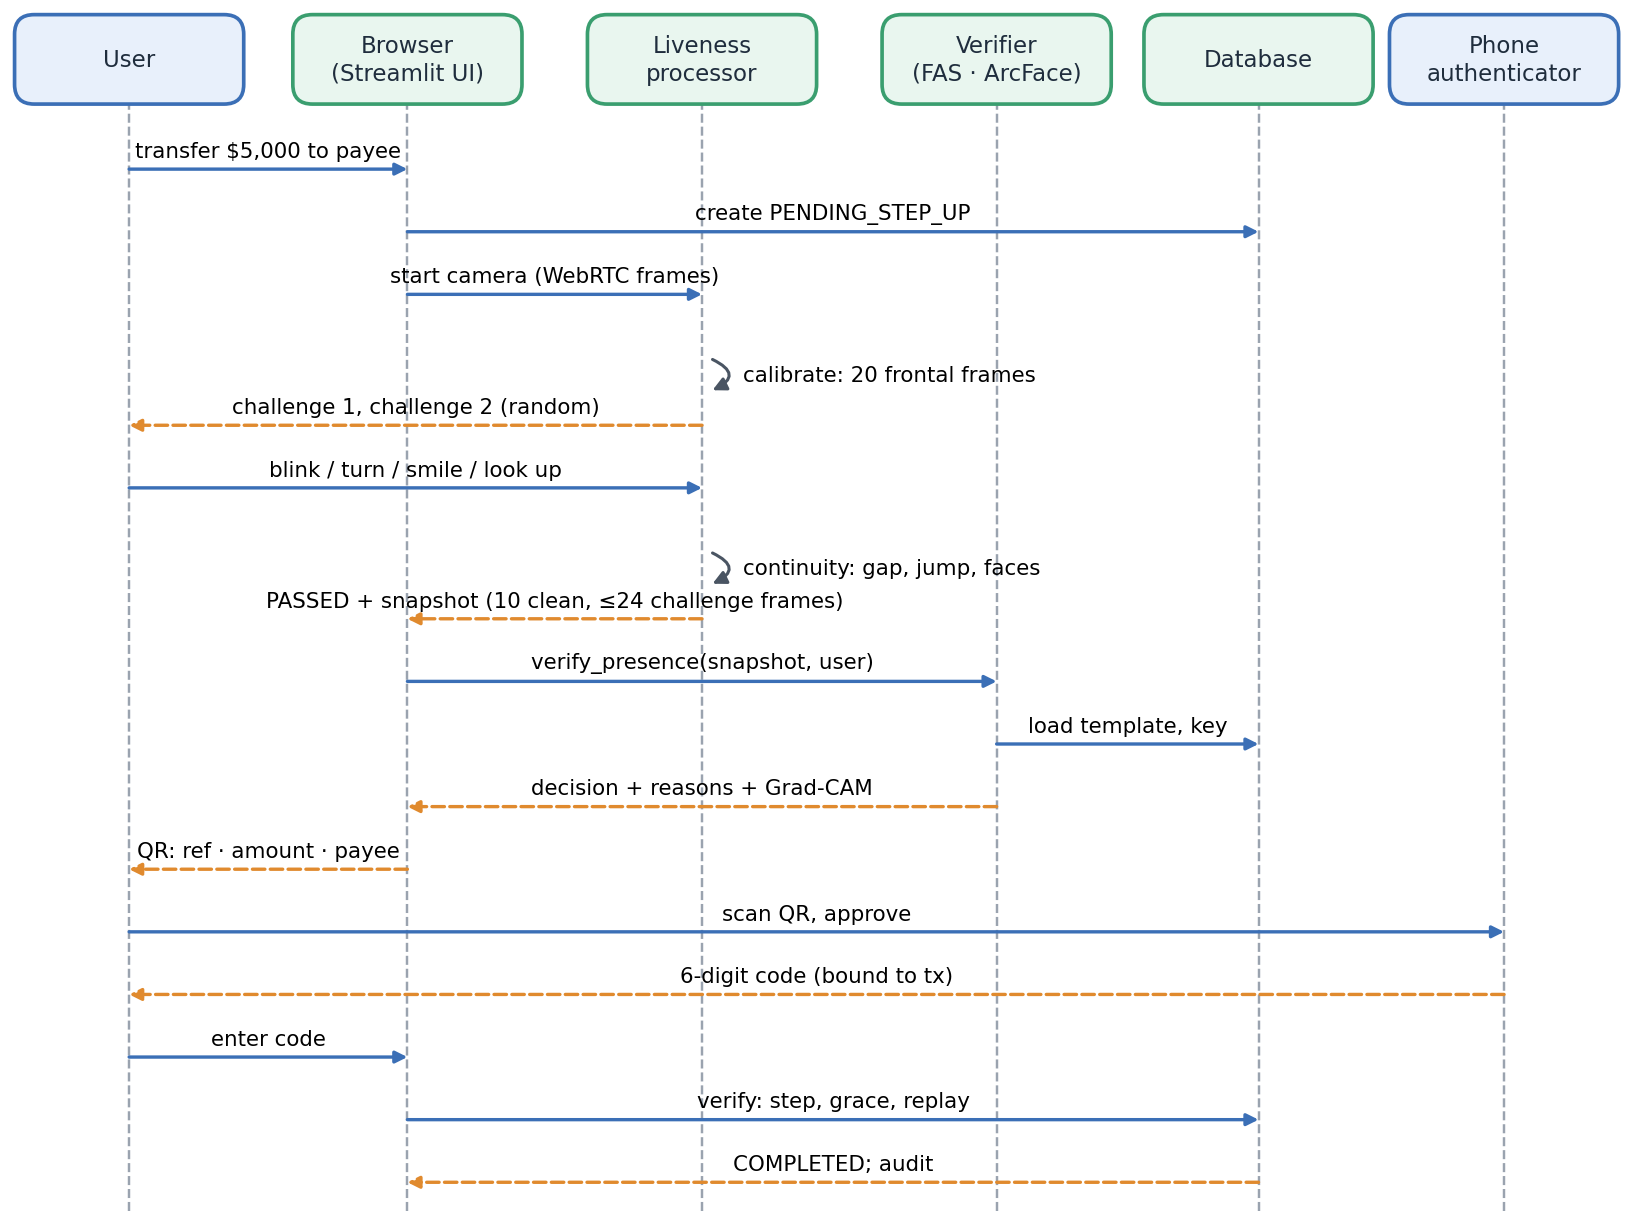
\includegraphics[width=0.78\textwidth]{figures/fig_sequence.png}
\caption{Step-up protocol for a high-value transfer. The presence check (calibration, two random
challenges, continuity, anti-spoofing and template match) precedes a transaction-bound code computed
offline by the paired phone.}
\label{fig:sequence}
\end{figure*}

\subsection{Randomized Active Liveness (L)}
\label{sec:liveness}
Each frame is processed by the MediaPipe Face Landmarker, which returns 478 landmarks, 52 expression
blendshape scores and a facial transformation matrix $\mathbf{R}$, on a 480-pixel-wide copy of the
frame. Head yaw and pitch (in degrees) are
\begin{equation}
\psi = \operatorname{atan2}(R_{02}, R_{22}), \qquad \theta = \arcsin(-R_{12}),
\end{equation}
the blink score $b$ is the mean of the left and right eye-blink blendshapes and the smile score $s$ the
mean of the two mouth-smile blendshapes.

\emph{Calibration.} The user first looks at the camera; 20 frontal frames ($|\psi|<15^\circ$,
$|\theta|<20^\circ$) are collected, every second one is kept, and the per-user baseline
$(\bar{\psi},\bar{\theta},\bar{b},\bar{s})$ is the median over these ten frames. Judging challenges
relative to the user's own neutral face makes them robust to camera placement and to people whose
resting expression is far from the population average.

\emph{Challenges.} Two distinct challenges are drawn at random from five, giving 20 ordered pairs, each
with a 9-s time limit:
\begin{itemize}
\item turn left or right: $|\psi-\bar{\psi}|>18^\circ$ in the requested (mirrored) direction;
\item look up: $\bar{\theta}-\theta>12^\circ$;
\item blink twice: $b>\max(0.45,\bar{b}+0.3)$ followed by $b<\max(0.25,\bar{b}+0.1)$, twice;
\item smile: $s>\max(0.45,\bar{s}+0.25)$.
\end{itemize}
The attempt fails on a timeout or if more than one face is in view.

\subsection{Presence Continuity}
\label{sec:continuity}
Baseline-relative liveness assumes that the face seen during calibration is the face that performs the
challenges. Our own red-team testing showed that this assumption can be violated
(Section~\ref{sec:res-swap}). We therefore enforce continuity at two levels.

\emph{Frame level.} Let $c_t$ be the face-box center, $w_t$ its width and $\Delta t$ the time since the
previous detected face. During calibration, any of $\Delta t>0.7$\,s, $\lVert c_t-c_{t-1}\rVert>0.5\,
w_{t-1}$, $\max(w_t/w_{t-1},w_{t-1}/w_t)>1.5$, or a second face restarts calibration and discards its
frames; during the challenges the same events fail the attempt. On genuine videos the largest observed
values were a shift of 0.03 face widths per frame and a gap of 0.07\,s, well inside these limits.

\emph{Decision level.} Every third challenge frame is sampled (at most 24). The server requires that
the ArcFace embeddings of three challenge frames have cosine similarity of at least 0.35 with the
calibration embedding, and that at least three neutral challenge frames
($|\Delta\psi|,|\Delta\theta|<10^\circ$, $b,s<0.5$) also pass PAD. Same-person similarities in our
data were 0.5--0.8 and different-person similarities below 0.25.

\subsection{Passive Presentation Attack Detection (F)}
\label{sec:pad}
The PAD network (Fig.~\ref{fig:fasnet}) has two ResNet-18~\cite{resnet} encoders initialized from
ImageNet. The spatial branch receives the RGB face crop (224$\times$224, ImageNet normalization); the
frequency branch receives the per-channel log-magnitude of the centered 2-D FFT~\cite{fft}, min--max
normalized. The two 512-D features are concatenated and passed through FC(256)--BatchNorm--ReLU--Dropout
(0.4)--FC(2). The network has 22.6\,M parameters. The face crop is the landmark bounding box with a
20\pct\ margin, identical in training and inference.

Training fine-tunes the last two residual stages of both encoders and the head with AdamW~\cite{adamw},
a one-cycle schedule (peak learning rates $10^{-4}$ for the encoders and $10^{-3}$ for the head),
cross-entropy with label smoothing 0.1, batches of 16 and 2,000 samples per epoch for three epochs,
selecting the epoch with the lowest validation ACER. Splits are by subject, so no person appears in two
splits. Webcam samples are weighted three times, and both classes receive the same augmentation
(random crop of 78--100\pct, flip, brightness, contrast and white-balance changes, downscaling to
35--80\pct, blur, gamma 1.2--1.8, sensor noise and JPEG quality 35--95), applied before both branches.
Without this, an early model learned that blurred faces are attacks.

At run time the score is the median REAL probability of ten clean calibration frames,
\begin{equation}
p_F=\operatorname{median}_{i=1,\dots,10} P(\text{real}\mid x_i), \qquad F = [\,p_F\ge\tau_F\,],
\end{equation}
where $\tau_F$ is the equal-error point on webcam validation clips (0.185 for the deployed model).

\begin{figure}[!t]
\centering
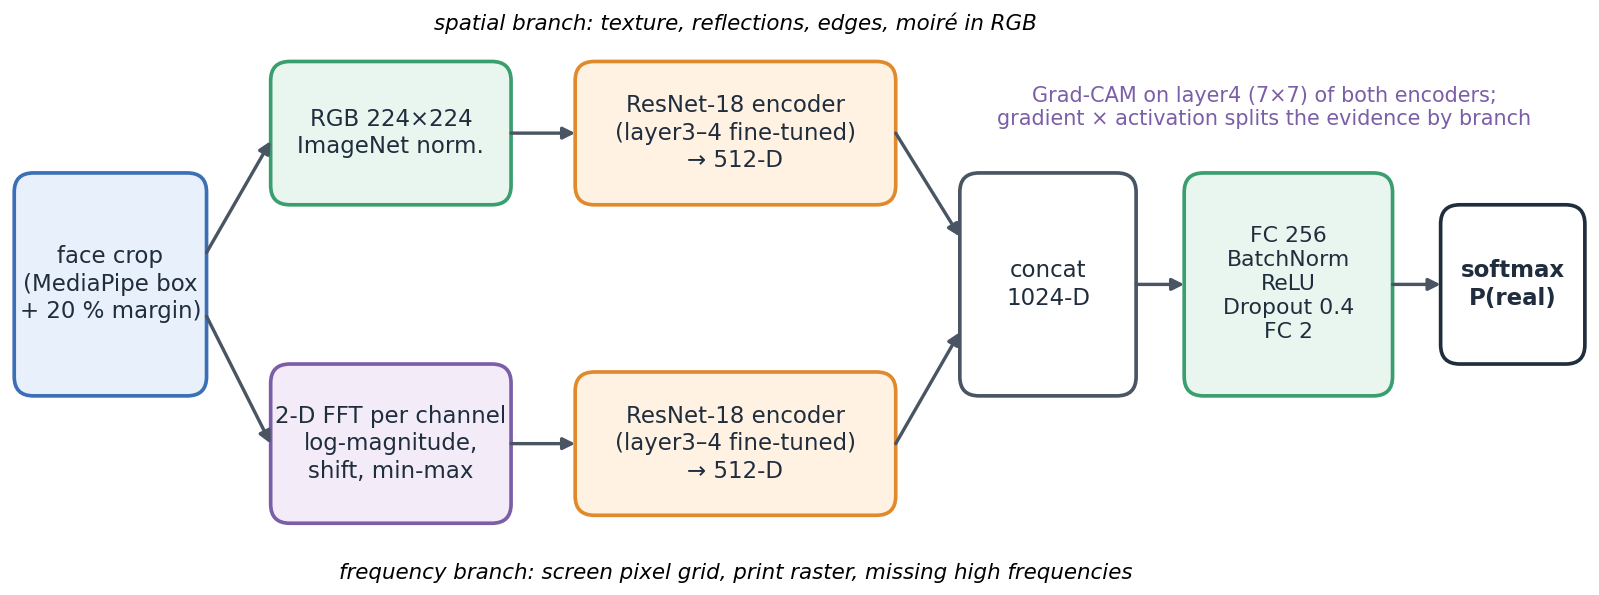
\includegraphics[width=\columnwidth]{figures/fig_fas_network.png}
\caption{Dual-branch spatial--frequency PAD network. Grad-CAM is computed on the last residual stage
of both encoders.}
\label{fig:fasnet}
\end{figure}

\subsection{Face Verification on a Cancelable Template (A)}
\label{sec:template}
Faces are detected and aligned by RetinaFace~\cite{retinaface} and embedded by an ArcFace~\cite{arcface}
ResNet-50 trained on WebFace600K (the InsightFace \texttt{buffalo\_l} models), giving a unit-norm
$\mathbf{e}\in\mathbb{R}^{512}$; a verification averages five frames. The raw embedding is never stored.
Instead, each user receives a random 256-bit key $k$, from which HMAC-SHA256 derives the initial value
$x_0\in(0.01,0.99)$ and parameter $r\in[3.99,3.9999]$ of the logistic map~\cite{may1976}
\begin{equation}
x_{n+1}=r\,x_n(1-x_n),
\end{equation}
which is iterated 500 times before use. In this chaotic regime the sequence is highly sensitive to $k$.
A first sequence gives a permutation $\pi$ of the 512 dimensions; a second fills a 512$\times$256
matrix whose QR decomposition yields $\mathbf{W}\in\mathbb{R}^{256\times512}$ with orthonormal rows.
The template and the match rule are
\begin{equation}
\mathbf{t}=\frac{\mathbf{W}\,\mathbf{e}_{\pi}}{\lVert\mathbf{W}\,\mathbf{e}_{\pi}\rVert},\qquad
A=[\,\mathbf{t}'^{\top}\mathbf{t}\ge 0.40\,],
\end{equation}
where $\mathbf{t}'$ is the protected probe (Fig.~\ref{fig:template}). An orthonormal projection
approximately preserves inner products~\cite{jl1984}, so accuracy is retained, while the 512-to-256
reduction is many-to-one. The 1,024-byte template is stored in clear; the key $k$ and the OTP secret
are encrypted at rest with Fernet (AES-128-CBC with HMAC-SHA256). Re-keying revokes a template.

\begin{figure}[!t]
\centering
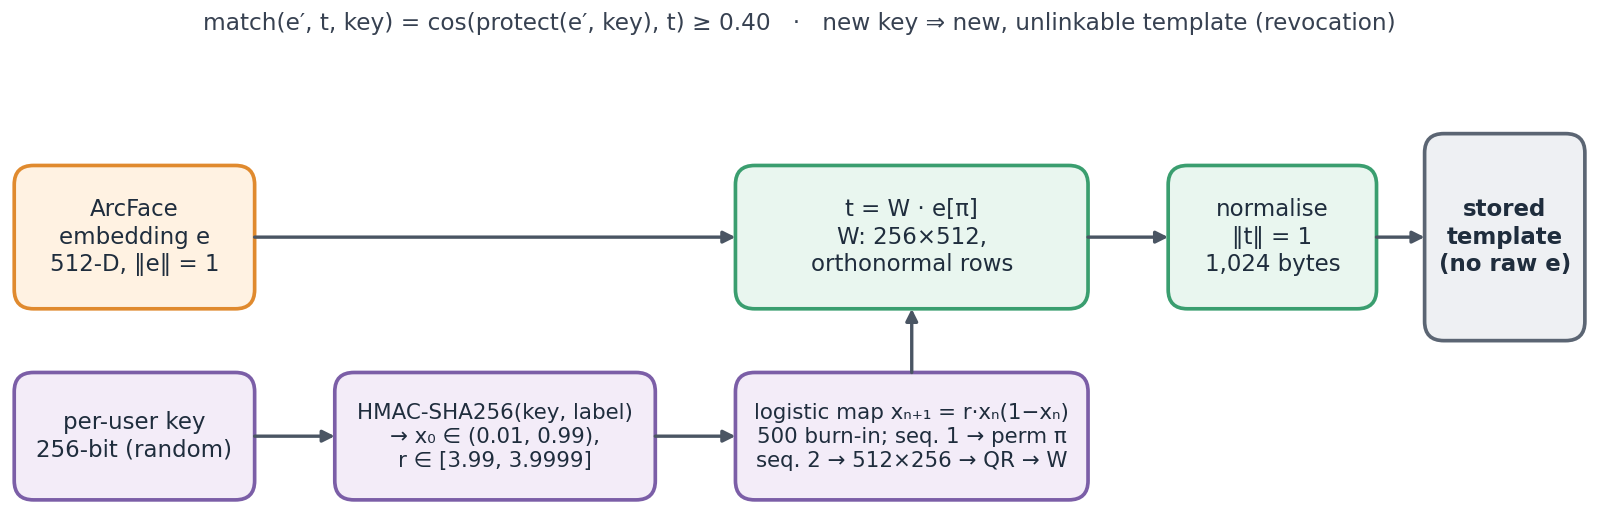
\includegraphics[width=\columnwidth]{figures/fig_template.png}
\caption{Cancelable template. A per-user key drives a logistic map that produces a permutation and an
orthonormal 512$\to$256 projection; a new key yields a new, unlinkable template.}
\label{fig:template}
\end{figure}

\subsection{Decision Fusion and Explanations}
The presence check passes only if all checks pass (Fig.~\ref{fig:fusion}):
\begin{equation}
D = L \wedge C \wedge F \wedge A,
\end{equation}
where $C$ denotes the continuity conditions of Section~\ref{sec:continuity}, and $F$ also requires the
challenge-frame PAD median to reach $\tau_F$ when measured. Every decision is accompanied by Grad-CAM
maps~\cite{gradcam} of both PAD encoders, a branch attribution (gradient $\times$ activation on the
fused 1024-D feature for $\text{logit}_\text{real}-\text{logit}_\text{spoof}$, summed per branch), the
radial power spectrum and high-frequency energy of the crop, its fractal dimension by differential box
counting~\cite{sarkar1994}, a liveness timeline, and plain-language reasons generated from these
numbers. All processing is local; no external service is called.

\begin{figure}[!t]
\centering
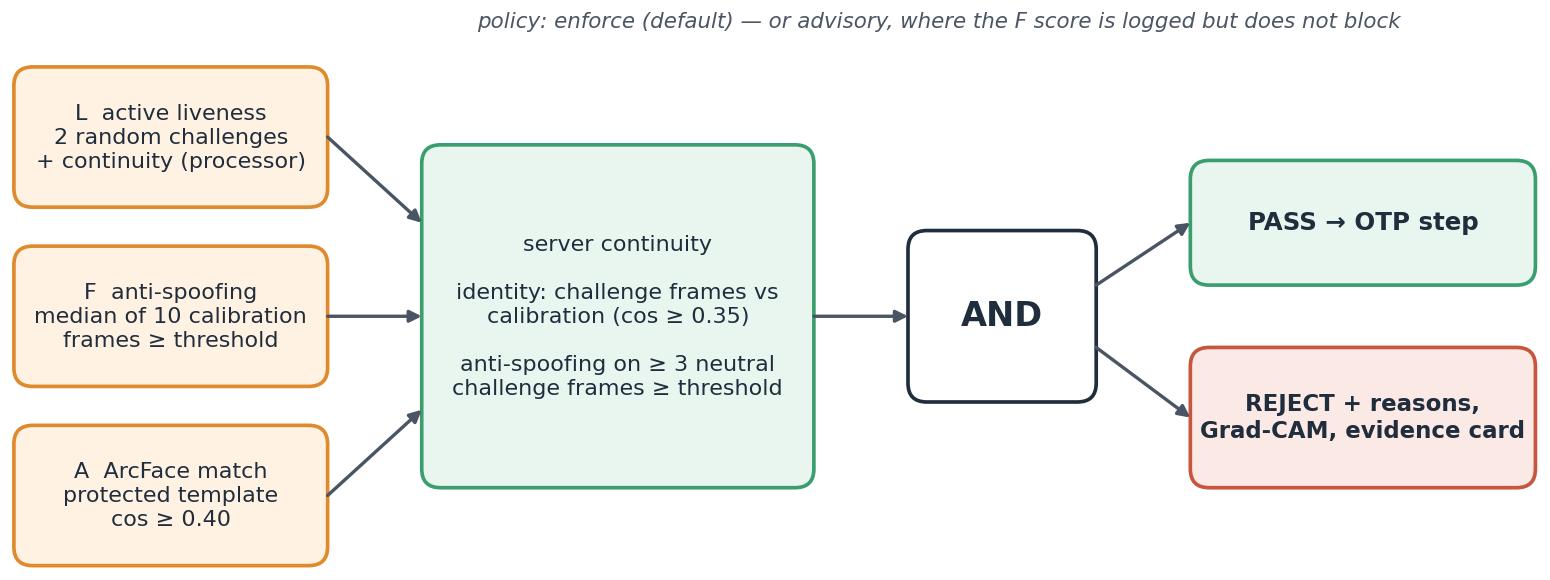
\includegraphics[width=\columnwidth]{figures/fig_fusion.png}
\caption{Decision fusion. Liveness, anti-spoofing and template match are combined by a logical AND
after the server-side continuity checks; a rejection is returned with its reasons and saliency maps.}
\label{fig:fusion}
\end{figure}

\subsection{Transaction-Bound Random-Walk OTP}
\label{sec:otp}
At pairing, the server generates a 256-bit secret $K$, shows it once in a QR code, and stores it
encrypted; the phone keeps it in browser storage. Let $T=\lfloor t/30\rfloor$ be the time step and
$\mathit{ctx}=\texttt{TX}|\mathit{ref}|\mathit{amount\_cents}|\mathit{payee}$ the transfer context. The
seed is
\begin{equation}
\sigma=\text{HMAC-SHA256}\big(K,\;T_{[8]}\,\Vert\,\text{SHA256}(\mathit{ctx})\big),
\end{equation}
and a byte stream $z_i=\text{SHA256}(\sigma\Vert i)$, $i=0,1,\dots$, supplies uniform choices by
rejection sampling. The walk runs on a public graph $G$: a 64-node ring lattice of degree 6 rewired with
probability 0.3 in the Watts--Strogatz manner~\cite{watts1998}, built deterministically from a public
seed (192 edges, connected, degrees 3--10, diameter 4). The walk chooses a start node $v_0$ uniformly
and then 16 uniformly chosen neighbors, $v_{j+1}\in N(v_j)$. The code is
\begin{equation}
\begin{split}
h&=\text{SHA256}(\texttt{walk-otp-v2}\,\Vert\,v_0\Vert\cdots\Vert v_{16}),\\
\mathit{OTP}&=\operatorname{DT}(h)\bmod 10^6,
\end{split}
\end{equation}
where $\operatorname{DT}$ is the dynamic truncation of RFC~4226~\cite{rfc4226} and node identifiers are
encoded as 16-bit integers (Fig.~\ref{fig:otp}). Because the seed includes $\mathrm{SHA256}(\mathit{ctx})$,
a code is valid only for the transfer shown on the phone, which implements dynamic
linking~\cite{psd2rts}.

The server accepts the current step, the previous step only within 10\,s of the step change, and the
next step only if the phone clock is at most 10\,s ahead. A table of used steps refuses any step at or
before the last accepted one for the same account and scope, and three wrong codes block the transfer.
The phone page implements SHA-256 and HMAC in plain JavaScript, because browsers disable the Web Crypto
API on non-HTTPS local-network pages; twelve fixed test vectors (graph, path and code) are identical in
the Python and JavaScript implementations.

\emph{A design pitfall.} The first version of the generator drew the walk from a general-purpose
pseudo-random generator and truncated the raw path bytes. The four-byte truncation window covered only
two node identifiers, so 20,000 random secrets produced only 768 distinct codes, and a code could be
guessed in about 800 attempts. The current design hashes the full path before truncation and derives all
randomness from the keyed seed.

\begin{figure}[!t]
\centering
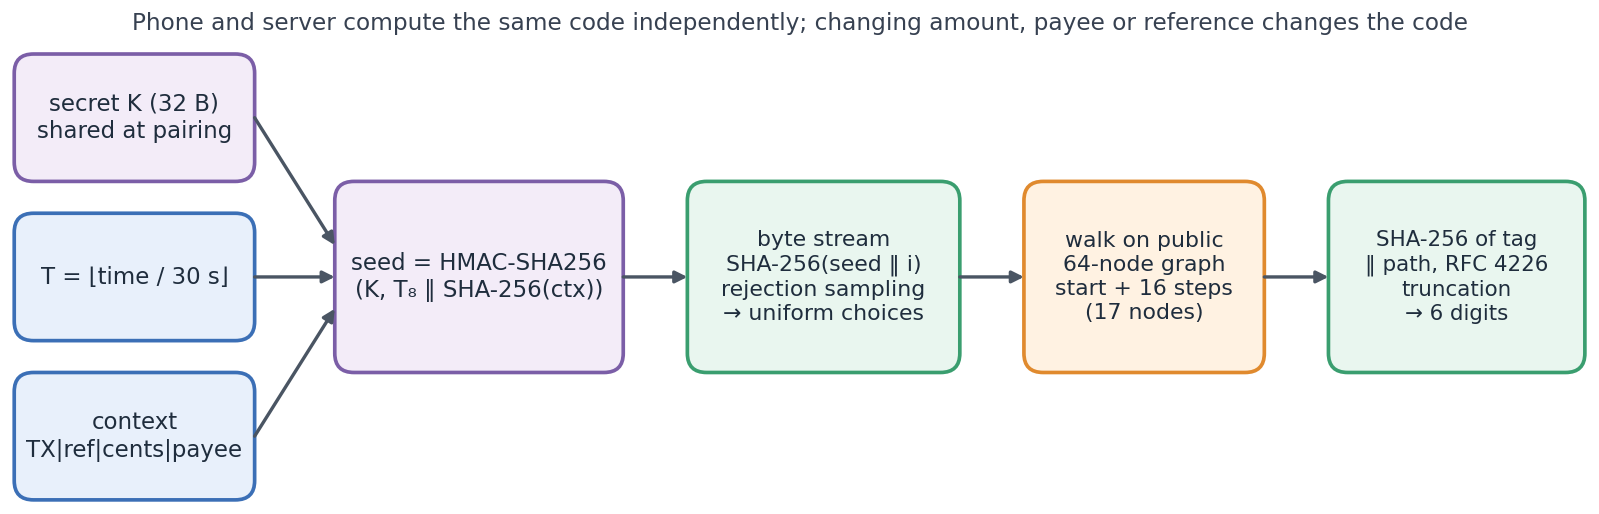
\includegraphics[width=\columnwidth]{figures/fig_otp_pipeline.png}
\caption{Transaction-bound random-walk OTP. Phone and server compute the code independently; changing
the amount, payee or reference changes the code.}
\label{fig:otp}
\end{figure}

% -----------------------------------------------------------------------------------------------------
\section{Experimental Setup}
\label{sec:setup}

\subsection{Data}
\emph{LCC-FASD.} We used the development subset of the Large Crowd-Collected Facial Anti-Spoofing
Dataset~\cite{lccfasd}: 416 genuine and 2,590 attack face crops from about 75 subjects, split by subject
into 52 training, 11 validation and 12 test groups (564 test frames, 103 genuine).

\emph{Webcam data.} Two authors recorded genuine videos and phone-replay attacks with the laptop webcam,
and the app saved ten crops per verification attempt. For the cross-person PAD analysis, the network was
retrained with one person entirely held out; that person's 50 genuine and 20 attack frames form the
unseen-person test set.

\emph{Field use.} Five enrolled users made 54 genuine verification attempts through the deployed
application between 8 and 12 October 2026.  %% TODO: describe the participants (team members / volunteers), their consent, and any ethics approval

\emph{Recorded attack.} A screen recording of a successful swap attack against an earlier version
(Section~\ref{sec:res-swap}) is kept as a regression test.

\subsection{Protocols}
\emph{Face verification:} 27 identities (25 from LCC-FASD, two webcam users), five enrolment images
each, 537 genuine probes and 13,962 impostor pairs; an attempt-level variant averages five frames (104
genuine, 2,704 impostor attempts). We also matched 986 attack presentations of enrolled identities
against their own templates.

\emph{Liveness:} the liveness processor was run offline on recorded videos at 15 frames per second with
the deployed thresholds. Replays were simulated by starting each challenge window at different offsets
in two phone-replay recordings; photo attacks used 15 photographs (ten LCC-FASD subjects and five
webcam images), presented still and with simulated tilts.

\emph{Swap simulation:} 360 sequences splice a photo of the victim for calibration with a live attacker
for the challenges, with transition gaps of 0, 0.3, 0.6, 1.0 and 1.5\,s.

\emph{System combinations:} we evaluated A, L, F and every AND-combination on five attempt categories:
genuine, zero-effort impostor, photo, replay and swap. A and F were measured jointly per attempt (up
to ten consecutive frames of one clip) with PAD models that had not seen the person. L acts on behavior,
which still frames lack, so it enters as the rate measured on video for that category and is combined
assuming independence. Metrics are reported over 1,000 weighted attempts (50\pct\ genuine, 12.5\pct\
for each attack category) drawn from 17 genuine, 442 impostor, and 58 each of photo, replay and swap
attempts.

\subsection{Metrics}
Following ISO/IEC 30107-3~\cite{iso30107}, the attack presentation classification error rate (APCER)
is the share of attacks accepted, the bona fide presentation classification error rate (BPCER) the share
of genuine presentations rejected, and $\text{ACER}=(\text{APCER}+\text{BPCER})/2$. For verification
we report the false accept rate (FAR), false reject rate (FRR) and equal error rate (EER). Proportions
are given with 95\pct\ Wilson score intervals where the sample is small.

\subsection{Implementation}
The system runs on a Windows 11 laptop CPU without a GPU  %% TODO: add CPU model and RAM
using Python 3.14, PyTorch 2.14, MediaPipe 0.10, InsightFace with ONNX Runtime 1.30 and Streamlit
1.64; the phone is a stock Android browser on the same Wi-Fi network. The suite of 105 automated tests
covers the OTP (including the cross-language vectors), liveness and continuity logic, the recorded
swap attack and 19 end-to-end application workflows.

% -----------------------------------------------------------------------------------------------------
\section{Results}
\label{sec:results}

\subsection{Face Verification and Template Protection}
\label{sec:res-face}
Table~\ref{tab:face} summarizes verification. In the protected domain, the EER was 0.25\pct\ and no
impostor pair was accepted at the 0.40 threshold (0 of 13,962; 95\pct\ upper bound 0.03\pct). The FRR
was 3.2\pct\ per frame and 0.96\pct\ (1 of 104) per five-frame attempt. Protection cost little
accuracy: protected and raw scores correlated at $r=0.969$ (mean absolute difference 0.033).

Template protection behaved as intended. The same face enrolled under two keys gave a mean cosine
similarity of $-0.002$ (largest magnitude 0.175, $n=133$), so templates under different keys are
unlinkable at the operating threshold, and none of 133 revoked templates matched its owner after
re-keying (highest score 0.194). Matching takes 3.8\,ms.

Recognition, however, is not liveness: 982 of 986 photo and replay presentations of enrolled identities
(99.6\pct; 95\pct\ CI 99.0--99.8\pct) matched their own template. This result motivates the
remaining components.

\begin{table}[!t]
\caption{Face Verification at Threshold 0.40}
\label{tab:face}
\centering
\footnotesize
\setlength{\tabcolsep}{4pt}
\begin{tabular}{lccc}
\toprule
 & Raw & Protected & Protected \\
 & (per frame) & (per frame) & (per attempt) \\
\midrule
Genuine / impostor & 537 / 13,962 & 537 / 13,962 & 104 / 2,704 \\
EER (\%) & 0.03 & 0.25 & 0.00 \\
FAR (\%) & 0.00 & 0.00 & 0.00 \\
FRR (\%) & 2.61 & 3.17 & 0.96 \\
TAR at FAR $=0.1\%$ (\%) & 100.0 & 99.8 & 100.0 \\
\bottomrule
\end{tabular}
\end{table}

\subsection{Active Liveness}
\label{sec:res-liveness}
A replayed video of natural behavior passed a blink-only challenge in all 12 trials, which confirms that
a single predictable challenge is insufficient. With two distinct random challenges, none of 240 replay
pairs passed (95\pct\ upper bound 1.6\pct), because the recordings did not contain the requested head
turns or smiles. No photo passed a challenge pair, either held still (0 of 45) or tilted (0 of 45;
upper bound 7.9\pct); a tilted photo passed a single look-up challenge once in 15 trials, which the
second challenge then caught.

On genuine recordings, the blink challenge was achieved in 29 of 32 windows (median 4.2\,s), and 20 of
26 genuine sequences passed with continuity enforced. In field use, 42 of 54 genuine attempts (77.8\pct;
95\pct\ CI 65.1--86.8\pct) passed liveness at the first try; the failures were timeouts on blinking (4),
turning right (4), turning left (2) and smiling (1), and one attempt with a second face in view. If
attempts are independent, 98.9\pct\ of users would pass within the three allowed attempts.

\subsection{Presentation Attack Detection}
\label{sec:res-pad}
Table~\ref{tab:pad} and Fig.~\ref{fig:roc} compare the fused network with a spatial-only network
trained identically, both with the test person held out. On the 12 unseen LCC-FASD subjects, the
frequency branch helped (AUC 0.950 versus 0.884). On the unseen webcam person, it hurt (AUC 0.751
versus 0.902). At the operating thresholds, the fused model rejected 44\pct\ of that person's genuine
frames, against 30\pct\ for the spatial model. Per attempt, both models blocked the person's phone
attacks but rejected two of five genuine attempts.

Earlier ablations trained on LCC-FASD alone point the same way: on its test subjects, the spatial
branch alone reached AUC 0.986, the fused model 0.970, the frequency branch alone 0.736, a logistic
regression on high-frequency energy 0.691, and one on fractal dimension 0.523, which is close to
chance. The first model we received reached AUC 1.000 on the same split only because its training set
included the test images; we report this as a reminder of how easily PAD results are inflated.

The explanations support this reading. On four held-out examples, the spatial branch carried the
decision (attribution $+1.09$ and $+2.22$ for genuine faces, $-3.26$ and $-4.20$ for replays), while the
frequency attribution was small and of inconsistent sign. The fractal dimension of genuine and attack
crops was nearly identical ($2.031\pm0.042$ versus $2.023\pm0.043$), so we show it as an explanatory
feature only and do not use it in any decision.

\begin{table}[!t]
\caption{PAD With the Test Person Held Out (Frame Level)}
\label{tab:pad}
\centering
\footnotesize
\setlength{\tabcolsep}{3pt}
\begin{tabular}{llcccccc}
\toprule
Test set & Model & $\tau_F$ & AUC & EER & APCER & BPCER & ACER \\
 & & & & (\%) & (\%) & (\%) & (\%) \\
\midrule
\multirow{2}{*}{LCC-FASD} & Spatial & 0.205 & 0.884 & 22.3 & 44.0 & 6.8 & 25.4 \\
 & Fused & 0.330 & 0.950 & 14.6 & 58.6 & 0.0 & 29.3 \\
\midrule
\multirow{2}{*}{Webcam} & Spatial & 0.205 & 0.902 & 20.0 & 10.0 & 30.0 & 20.0 \\
 & Fused & 0.330 & 0.751 & 29.0 & 25.0 & 44.0 & 34.5 \\
\bottomrule
\end{tabular}
\\[3pt]
\parbox{\columnwidth}{\footnotesize LCC-FASD: 564 frames (103 genuine) from 12 unseen subjects.
Webcam: 70 frames (50 genuine) from one unseen person. Thresholds were set on webcam validation clips,
which explains the high APCER on LCC-FASD.}
\end{table}

\begin{figure}[!t]
\centering
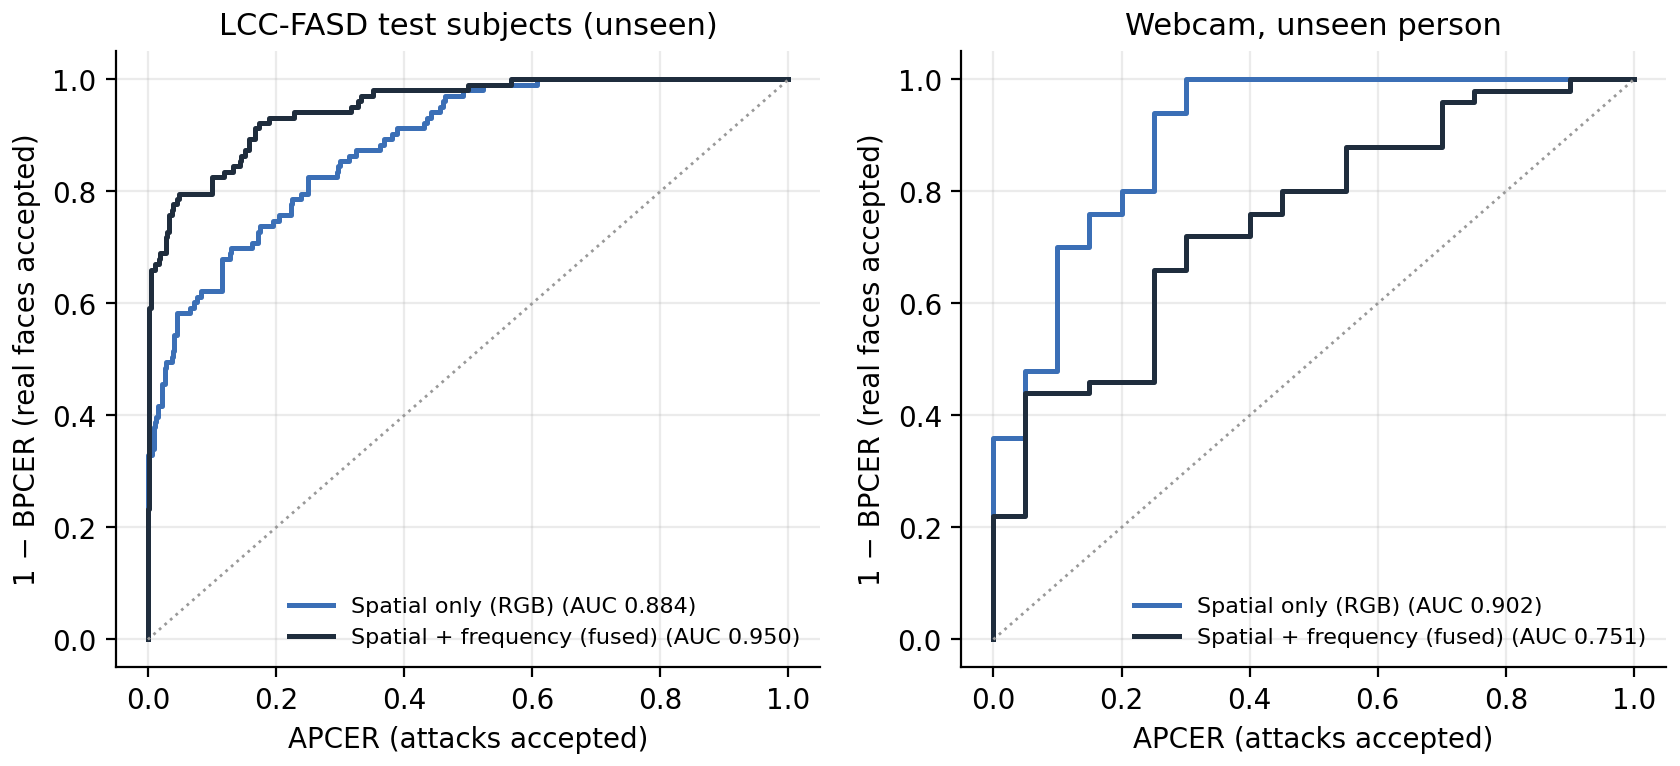
\includegraphics[width=\columnwidth]{figures/fig_fas_roc.png}
\caption{ROC curves of the spatial-only and fused PAD networks on unseen LCC-FASD subjects (left) and
an unseen webcam user (right).}
\label{fig:roc}
\end{figure}

\subsection{Component Combinations}
\label{sec:res-system}
Fig.~\ref{fig:heatmap} gives the acceptance rate of every combination for every attempt category, and
Table~\ref{tab:combo} the aggregate metrics. Each component alone has a blind spot: A rejects impostors
but accepts 98.3\pct\ of photo, replay and swap attempts; L rejects photos and replays but accepts
77.8\pct\ of impostors, who are live; F alone accepts 48.3\pct\ of presentation attacks and does not
address impostors at all. A+L was the best combination by F1 (0.845) and accepted no attack of any type.
Adding F kept the attack acceptance at zero but rejected more genuine attempts (64.1\pct\ accepted
versus 73.2\pct). F nevertheless provides defense in depth: if liveness were bypassed, for instance by
a video that can respond to prompts, A+F would still block 51.7\pct\ of re-imaged faces.

\begin{figure}[!t]
\centering
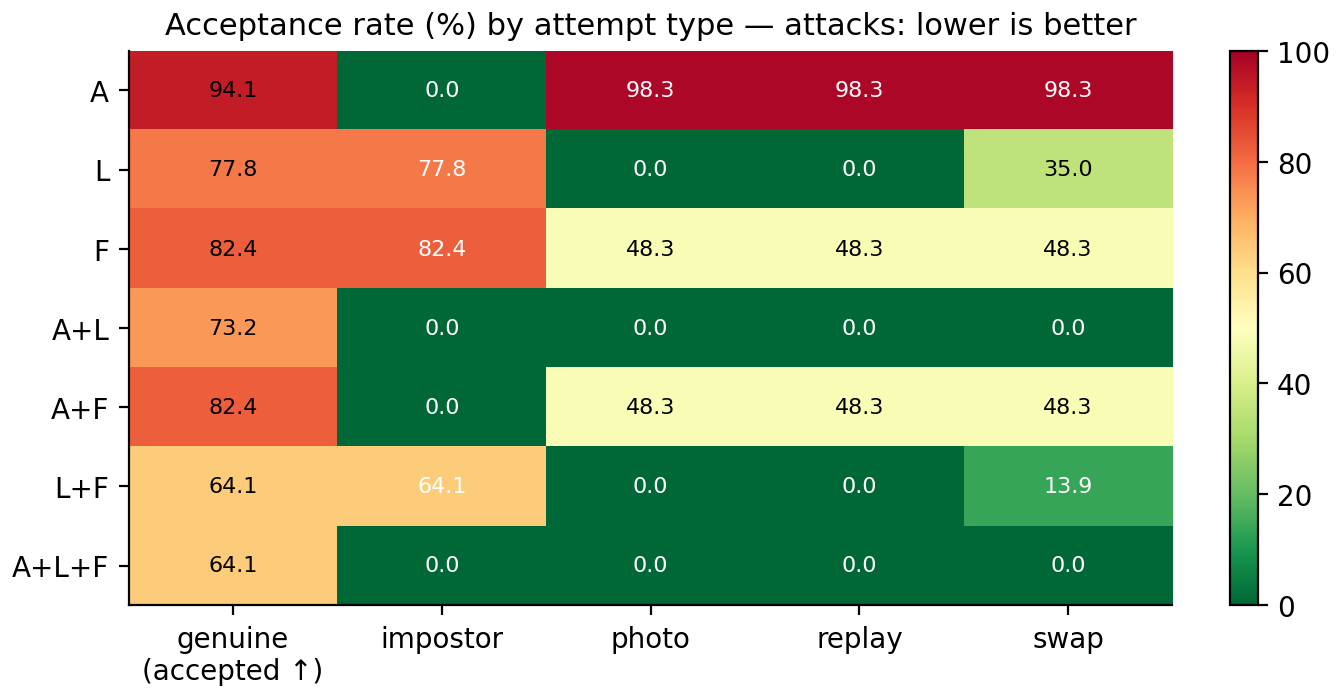
\includegraphics[width=\columnwidth]{figures/fig_combo_heatmap.png}
\caption{Acceptance rate (\%) of each component combination by attempt category. Genuine: higher is
better; attacks: lower is better.}
\label{fig:heatmap}
\end{figure}

\begin{table}[!t]
\caption{Component Combinations Over 1,000 Weighted Attempts}
\label{tab:combo}
\centering
\footnotesize
\setlength{\tabcolsep}{3.5pt}
\begin{tabular}{lcccccc}
\toprule
Checks & Acc. & Prec. & Recall & F1 & APCER$_{\max}$ & BPCER \\
 & (\%) & (\%) & (\%) & & (\%) & (\%) \\
\midrule
A & 60.2 & 56.1 & 94.1 & 0.703 & 98.3 & 5.9 \\
L & 74.8 & 73.4 & 77.8 & 0.755 & 77.8 & 22.2 \\
F & 62.8 & 59.2 & 82.4 & 0.689 & 82.4 & 17.6 \\
A+L & \textbf{86.6} & 100.0 & 73.2 & \textbf{0.845} & 0.0 & 26.8 \\
A+F & 73.1 & 69.5 & 82.4 & 0.754 & 48.3 & 17.6 \\
L+F & 72.3 & 76.7 & 64.1 & 0.698 & 64.1 & 35.9 \\
A+L+F & 82.0 & 100.0 & 64.1 & 0.781 & 0.0 & 35.9 \\
\bottomrule
\end{tabular}
\\[3pt]
\parbox{\columnwidth}{\footnotesize Positive class: genuine. APCER$_{\max}$: highest acceptance over the
impostor, photo, replay and swap categories. Weights: 50\pct\ genuine, 12.5\pct\ per attack category.}
\end{table}

\subsection{The Calibration-Swap Attack}
\label{sec:res-swap}
While testing our own deployment, we found that an attacker could hold a phone showing the victim
close to the camera during calibration and then remove it and perform the challenges with their own
live face. Calibration frames then show the victim, so A passes; the challenges are performed by a live
person, so L passes; and F is scored on calibration frames, where the PAD model then deployed gave the
phone a REAL probability of 0.72, above its threshold. The attack succeeded.

Fig.~\ref{fig:swap} shows the effect of the continuity defense of Section~\ref{sec:continuity}. Before
it, swaps were accepted in 76.4\pct\ of attempts by A+L and in 37.5\pct\ by A+L+F; with it, both fell to
0\pct. In the 360 simulated sequences, continuity alone stopped every swap with a transition gap of
1.0\,s or more and half of those with shorter gaps; the identity check on challenge frames rejected the
remainder, because no impostor's challenge frames matched the victim's calibration embedding. The
recorded attack contains a 0.94-s gap and a jump of 0.9 face widths and is now rejected at the moment
the phone is removed. We also retrained the PAD model with this attack, after which it scored the phone
0.03.

\begin{figure}[!t]
\centering
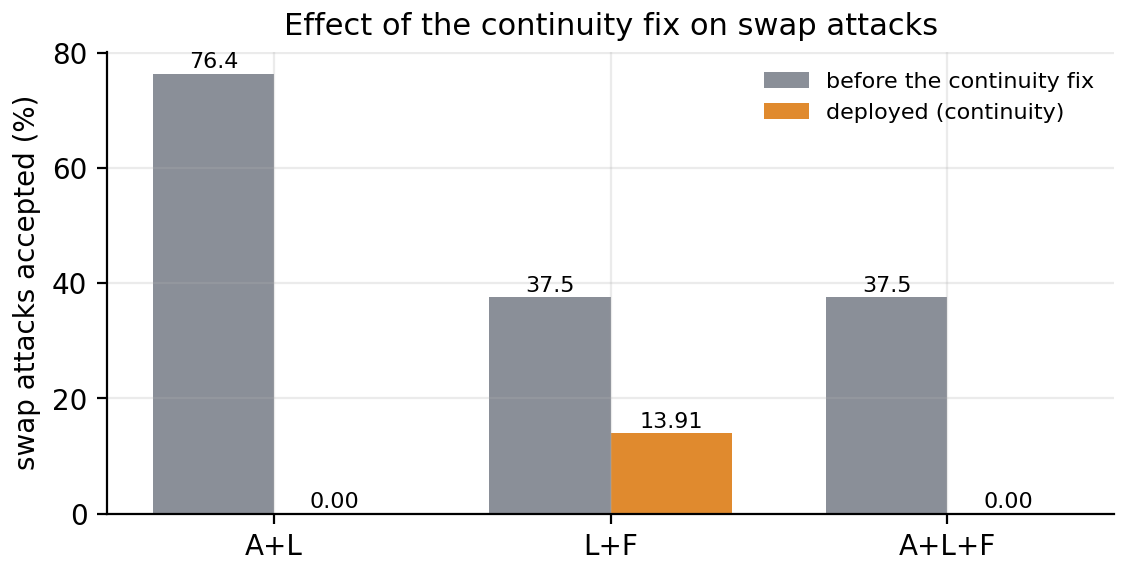
\includegraphics[width=\columnwidth]{figures/fig_swap.png}
\caption{Swap attacks accepted before and after the presence-continuity defense.}
\label{fig:swap}
\end{figure}

\subsection{Transaction-Bound OTP}
\label{sec:res-otp}
Table~\ref{tab:otp} summarizes the OTP analysis. From 20,000 random secrets at a fixed time step, the
walk produced 19,781 distinct codes, against 19,790 for RFC~6238 TOTP and an expected 19,801 for an
ideal uniform generator; the earlier design produced 768. Over 200,000 codes, a $\chi^2$ test on 100
equal buckets gave $p=0.14$ (Fig.~\ref{fig:uniformity}), and the six digit positions gave $p$ between
0.20 and 0.83.

Binding was complete in our tests: across 5,000 trials each, flipping one key bit, advancing the time
step, changing the amount by one cent, or changing the payee or reference never reproduced the code,
and on average 5.38--5.41 of the six digits changed, against 5.4 expected for independent codes. The
walk itself has about $2^{47.4}$ possible paths, more than the $2^{19.9}$ code space, so the output
entropy is limited by the six-digit format rather than by the graph. With three tries per transfer, a
guessing attacker succeeds with probability $3\times10^{-6}$ (at most $6\times10^{-6}$ during the grace
window, when two codes are valid). Generating a code takes 1.9\,ms (0.06\,ms with the graph cached),
against 0.008\,ms for TOTP.

\begin{table}[!t]
\caption{Random-Walk OTP Analysis}
\label{tab:otp}
\centering
\footnotesize
\setlength{\tabcolsep}{4pt}
\begin{tabular}{lc}
\toprule
Property & Value \\
\midrule
Distinct codes, 20,000 secrets (walk / TOTP / ideal) & 19,781 / 19,790 / 19,801 \\
Distinct codes, earlier truncation design & 768 \\
$\chi^2$ uniformity, 200,000 codes, 100 buckets & $p=0.14$ \\
Same code after 1-cent, payee or 1-bit key change & 0 / 5,000 each \\
Digits changed on any input change (ideal 5.4) & 5.38--5.41 \\
Seed avalanche (share of bits flipped) & 0.500 \\
Graph: nodes, edges, diameter, mean path & 64, 192, 4, 2.49 \\
Guess success per transfer (3 tries) & $3\times10^{-6}$ \\
Generation time (graph cached) & 1.9\,ms (0.06\,ms) \\
\bottomrule
\end{tabular}
\end{table}

\begin{figure}[!t]
\centering
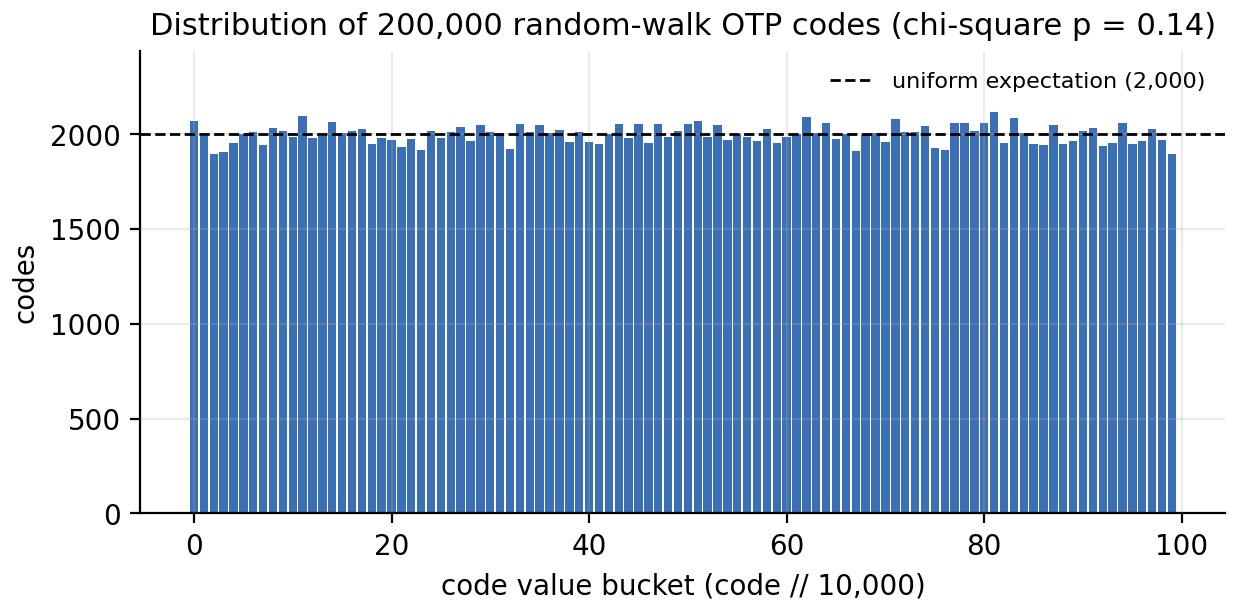
\includegraphics[width=\columnwidth]{figures/fig_otp_uniformity.png}
\caption{Distribution of 200,000 random-walk codes in 100 equal buckets.}
\label{fig:uniformity}
\end{figure}

\subsection{Latency}
\label{sec:res-latency}
Liveness runs on every camera frame: landmark extraction takes 11.2\,ms and 17.9\,ms with the user
overlay, within the 66.7-ms budget of 15 frames per second. The server-side presence verification took
4.2\,s at best and 4.8\,s on average on mains power, and 8.1\,s on average when the same laptop ran on
battery. In the battery measurement, ArcFace detection, alignment and embedding of the five calibration
and three challenge frames accounted for 5.8\,s, the PAD network for 1.5\,s, face cropping for 0.4\,s
and the explanation for 0.4\,s; template matching took 0.1\,ms. ArcFace is therefore the bottleneck,
and fewer or pre-cropped frames, or a GPU, would shorten the wait.

% -----------------------------------------------------------------------------------------------------
\section{Discussion}
\label{sec:discussion}

\subsection{Why Heterogeneous Checks Must Be Combined}
The combination study shows that the three face checks are complementary rather than redundant. A
answers ``who'', L answers ``is it live'', and neither answers the other's question; A alone accepted
almost every presentation attack, and L alone accepted almost every impostor. The swap attack shows the
corollary: when the checks look at different moments of the session, an attacker can satisfy each one
with a different face. A secure composition must therefore bind the checks to the same continuous
presence, not merely require each to pass.

\subsection{The Cost of Defense in Depth}
On our test set, adding F to A+L did not block any additional attack but lowered genuine acceptance from
73.2\pct\ to 64.1\pct, and 7 of 54 field attempts were rejected by PAD. We keep F because our attack set
does not contain videos that respond to prompts, and against those F is the remaining layer. A bank
could make this trade-off explicit, for example by enforcing F only above a second, higher amount.

\subsection{Generalization of the Frequency Branch}
The frequency branch improved in-domain AUC and reduced cross-person AUC. A plausible explanation is
that Fourier-domain features capture camera- and compression-specific artifacts that differ between
datasets and devices, in line with the generalization problem reported in the
literature~\cite{ssdg,fas_survey}. A spatial-first model, or domain-generalization training, is the
natural next step; our results do not support adding a frequency branch for webcam deployment without
cross-device data.

\subsection{Lessons From Building the System}
Three defects were found only because we tested the integrated system adversarially and with
explanations: the swap attack, the memorizing PAD model whose test images were in its training set, and
the OTP truncation that collapsed the code space to 768 values. Explanations exposed a bias of an early
PAD model that rejected blurred and backlit genuine faces. We think these lessons transfer to other
biometric payment systems: test each joint between components, keep strict subject-wise splits, and
measure the output distribution of any custom OTP construction.

\subsection{Limitations}
\label{sec:limits}
The webcam data come from two people, the field use from five users and 54 attempts, and the
cross-person PAD test from one held-out person with 17 held-out genuine attempts in total; the
corresponding confidence intervals are wide. We did not evaluate on public PAD benchmarks such as
OULU-NPU, so our PAD numbers are not directly comparable with~\cite{cdcn,ssdg}. The liveness evaluation
uses recorded videos; a replay crafted to contain every challenge, a real-time deepfake, or frames
injected through a virtual camera are outside our threat model. The system-level combination assumes
that liveness is independent of A and F. The phone key is held in browser storage and served over
plain HTTP on the local network, and template irreversibility depends on the secrecy of the per-user
key~\cite{kong2006}. Finally, we did not run a formal usability study.

% -----------------------------------------------------------------------------------------------------
\section{Conclusion}
\label{sec:conclusion}
We presented a step-up authentication system for high-value transfers that binds a live, genuine and
matching face and a phone-computed code to a single transaction. Face recognition alone accepted 99.6\pct\
of photo and replay presentations of the enrolled user; combining it with randomized liveness rejected
every impostor, photo, replay and swap attempt in our tests. We identified a calibration-swap attack that
defeated all three face checks in 37.5\pct\ of simulated attempts and removed it with a
presence-continuity check. The cancelable template retained accuracy (0.25\pct\ EER, no false accepts in
13,962 impostor pairs) while being revocable and unlinkable, and the transaction-bound random-walk OTP
was as uniform as TOTP while satisfying dynamic linking. Future work will evaluate PAD on public
benchmarks and with more people in leave-one-person-out protocols, move liveness into the browser,
detect camera-injection attacks, and study usability with a larger group of users.

% -----------------------------------------------------------------------------------------------------
\section*{Acknowledgment}
The authors thank the volunteers who tested the prototype.  %% TODO: adjust
%% IEEE Access requires disclosure of AI-generated text; keep and adapt this sentence.
The authors used Claude (Anthropic) to help draft and edit the text of this article; the authors
reviewed and revised all content and take full responsibility for it.  %% TODO: name the sections, per IEEE policy

% -----------------------------------------------------------------------------------------------------
\begin{thebibliography}{00}

\bibitem{psd2rts} European Commission, ``Commission Delegated Regulation (EU) 2018/389 of 27 November
2017 supplementing Directive (EU) 2015/2366 with regard to regulatory technical standards for strong
customer authentication and common and secure open standards of communication,'' \emph{Official Journal
of the European Union}, L 69, 2018.

\bibitem{arcface} J. Deng, J. Guo, N. Xue, and S. Zafeiriou, ``ArcFace: Additive angular margin loss
for deep face recognition,'' in \emph{Proc. IEEE/CVF Conf. Comput. Vis. Pattern Recognit. (CVPR)},
2019, pp. 4690--4699.

\bibitem{iso30107} \emph{Information Technology---Biometric Presentation Attack Detection---Part 3:
Testing and Reporting}, ISO/IEC 30107-3:2017, 2017.

\bibitem{fas_survey} Z. Yu, Y. Qin, X. Li, C. Zhao, Z. Lei, and G. Zhao, ``Deep learning for face
anti-spoofing: A survey,'' \emph{IEEE Trans. Pattern Anal. Mach. Intell.}, vol. 45, no. 5,
pp. 5609--5631, May 2023, doi: 10.1109/TPAMI.2022.3215850.

\bibitem{cdcn} Z. Yu, C. Zhao, Z. Wang, Y. Qin, Z. Su, X. Li, F. Zhou, and G. Zhao, ``Searching central
difference convolutional networks for face anti-spoofing,'' in \emph{Proc. IEEE/CVF Conf. Comput. Vis.
Pattern Recognit. (CVPR)}, 2020, pp. 5295--5305.

\bibitem{ssdg} Y. Jia, J. Zhang, S. Shan, and X. Chen, ``Single-side domain generalization for face
anti-spoofing,'' in \emph{Proc. IEEE/CVF Conf. Comput. Vis. Pattern Recognit. (CVPR)}, 2020,
pp. 8484--8493.

\bibitem{pan2007} G. Pan, L. Sun, Z. Wu, and S. Lao, ``Eyeblink-based anti-spoofing in face
recognition from a generic webcamera,'' in \emph{Proc. IEEE 11th Int. Conf. Comput. Vis. (ICCV)}, 2007,
pp. 1--8, doi: 10.1109/ICCV.2007.4409068.

\bibitem{ratha2001} N. K. Ratha, J. H. Connell, and R. M. Bolle, ``Enhancing security and privacy in
biometrics-based authentication systems,'' \emph{IBM Syst. J.}, vol. 40, no. 3, pp. 614--634, 2001.

\bibitem{iso24745} \emph{Information Security, Cybersecurity and Privacy Protection---Biometric
Information Protection}, ISO/IEC 24745:2022, 2022.

\bibitem{li2004} J. Li, Y. Wang, T. Tan, and A. K. Jain, ``Live face detection based on the analysis of
Fourier spectra,'' in \emph{Biometric Technology for Human Identification}, Proc. SPIE, vol. 5404,
2004, pp. 296--303, doi: 10.1117/12.541955.

\bibitem{boulkenafet2016} Z. Boulkenafet, J. Komulainen, and A. Hadid, ``Face spoofing detection using
colour texture analysis,'' \emph{IEEE Trans. Inf. Forensics Security}, vol. 11, no. 8,
pp. 1818--1830, Aug. 2016.

\bibitem{liu2018} Y. Liu, A. Jourabloo, and X. Liu, ``Learning deep models for face anti-spoofing:
Binary or auxiliary supervision,'' in \emph{Proc. IEEE/CVF Conf. Comput. Vis. Pattern Recognit.
(CVPR)}, 2018, pp. 389--398.

\bibitem{deeppixbis} A. George and S. Marcel, ``Deep pixel-wise binary supervision for face
presentation attack detection,'' in \emph{Proc. Int. Conf. Biometrics (ICB)}, 2019.

\bibitem{facedes} A. Jourabloo, Y. Liu, and X. Liu, ``Face de-spoofing: Anti-spoofing via noise
modeling,'' in \emph{Proc. Eur. Conf. Comput. Vis. (ECCV)}, 2018, pp. 290--306.

\bibitem{kollreider2007} K. Kollreider, H. Fronthaler, M. I. Faraj, and J. Bigun, ``Real-time face
detection and motion analysis with application in `liveness' assessment,'' \emph{IEEE Trans. Inf.
Forensics Security}, vol. 2, no. 3, pp. 548--558, Sep. 2007, doi: 10.1109/TIFS.2007.902037.

\bibitem{ear2016} T. Soukupov\'{a} and J. \v{C}ech, ``Real-time eye blink detection using facial
landmarks,'' in \emph{Proc. 21st Comput. Vis. Winter Workshop (CVWW)}, Rimske Toplice, Slovenia, 2016.

\bibitem{kartynnik2019} Y. Kartynnik, A. Ablavatski, I. Grishchenko, and M. Grundmann, ``Real-time
facial surface geometry from monocular video on mobile GPUs,'' 2019, \emph{arXiv:1907.06724}.

\bibitem{biohashing} A. B. J. Teoh, D. C. L. Ngo, and A. Goh, ``Biohashing: Two factor authentication
featuring fingerprint data and tokenised random number,'' \emph{Pattern Recognit.}, vol. 37, no. 11,
pp. 2245--2255, 2004.

\bibitem{kong2006} A. Kong, K.-H. Cheung, D. Zhang, M. Kamel, and J. You, ``An analysis of BioHashing
and its variants,'' \emph{Pattern Recognit.}, vol. 39, no. 7, pp. 1359--1368, 2006.  %% TODO: verify volume/issue/pages against the paper

\bibitem{rfc4226} D. M'Raihi, M. Bellare, F. Hoornaert, D. Naccache, and O. Ranen, ``HOTP: An
HMAC-based one-time password algorithm,'' IETF RFC 4226, Dec. 2005.

\bibitem{rfc6238} D. M'Raihi, S. Machani, M. Pei, and J. Rydell, ``TOTP: Time-based one-time password
algorithm,'' IETF RFC 6238, May 2011.

\bibitem{nist80063b} P. A. Grassi \emph{et al.}, ``Digital identity guidelines: Authentication and
lifecycle management,'' NIST Special Publication 800-63B, 2017.

\bibitem{gradcam} R. R. Selvaraju, M. Cogswell, A. Das, R. Vedantam, D. Parikh, and D. Batra,
``Grad-CAM: Visual explanations from deep networks via gradient-based localization,'' in \emph{Proc.
IEEE Int. Conf. Comput. Vis. (ICCV)}, 2017, pp. 618--626.

\bibitem{sequeira2021} A. F. Sequeira, T. Gon\c{c}alves, W. Silva, J. R. Pinto, and J. S. Cardoso,
``An exploratory study of interpretability for face presentation attack detection,'' \emph{IET
Biometrics}, vol. 10, no. 4, pp. 441--455, 2021, doi: 10.1049/bme2.12045.

\bibitem{pan2022} S. Pan, S. Hoque, and F. Deravi, ``An attention-guided framework for explainable
biometric presentation attack detection,'' \emph{Sensors}, vol. 22, no. 9, Art. no. 3365, 2022.

\bibitem{resnet} K. He, X. Zhang, S. Ren, and J. Sun, ``Deep residual learning for image
recognition,'' in \emph{Proc. IEEE Conf. Comput. Vis. Pattern Recognit. (CVPR)}, 2016, pp. 770--778.

\bibitem{fft} J. W. Cooley and J. W. Tukey, ``An algorithm for the machine calculation of complex
Fourier series,'' \emph{Math. Comput.}, vol. 19, pp. 297--301, 1965.

\bibitem{adamw} I. Loshchilov and F. Hutter, ``Decoupled weight decay regularization,'' in \emph{Proc.
Int. Conf. Learn. Represent. (ICLR)}, 2019.

\bibitem{retinaface} J. Deng, J. Guo, E. Ververas, I. Kotsia, and S. Zafeiriou, ``RetinaFace:
Single-shot multi-level face localisation in the wild,'' in \emph{Proc. IEEE/CVF Conf. Comput. Vis.
Pattern Recognit. (CVPR)}, 2020.

\bibitem{may1976} R. M. May, ``Simple mathematical models with very complicated dynamics,''
\emph{Nature}, vol. 261, pp. 459--467, 1976.

\bibitem{jl1984} W. B. Johnson and J. Lindenstrauss, ``Extensions of Lipschitz mappings into a Hilbert
space,'' \emph{Contemp. Math.}, vol. 26, pp. 189--206, 1984.

\bibitem{sarkar1994} N. Sarkar and B. B. Chaudhuri, ``An efficient differential box-counting approach
to compute fractal dimension of image,'' \emph{IEEE Trans. Syst., Man, Cybern.}, vol. 24, no. 1,
pp. 115--120, Jan. 1994, doi: 10.1109/21.259692.

\bibitem{watts1998} D. J. Watts and S. H. Strogatz, ``Collective dynamics of `small-world' networks,''
\emph{Nature}, vol. 393, pp. 440--442, 1998.

\bibitem{lccfasd} D. Timoshenko, K. Simonchik, V. Shutov, P. Zhelezneva, and V. Grishkin, ``Large
crowdcollected facial anti-spoofing dataset,'' in \emph{Proc. Comput. Sci. Inf. Technol. (CSIT)}, 2019,
pp. 123--126, doi: 10.1109/CSITechnol.2019.8895208.

\end{thebibliography}

% -----------------------------------------------------------------------------------------------------
%% TODO: IEEE Access requires a biography (and a photo, optional) for EVERY author.
\begin{IEEEbiographynophoto}{Nilay Kant Shahi} is pursuing the B.Tech. degree in information
technology at Vellore Institute of Technology, Vellore, India. Research interests include
biometric authentication, presentation attack detection and applied cryptography.  %% TODO: author to rewrite in their own words
\end{IEEEbiographynophoto}

\begin{IEEEbiographynophoto}{Magizharasan K} is pursuing the B.Tech. degree in information technology
at Vellore Institute of Technology, Vellore, India.  %% TODO
\end{IEEEbiographynophoto}

\begin{IEEEbiographynophoto}{Rwitankar Giri} is pursuing the B.Tech. degree in information technology
at Vellore Institute of Technology, Vellore, India.  %% TODO
\end{IEEEbiographynophoto}

\begin{IEEEbiographynophoto}{Mohanraj G} is with the School of Computer Science Engineering and
Information Systems, Vellore Institute of Technology, Vellore, India.  %% TODO
\end{IEEEbiographynophoto}

\EOD

\end{document}
